\documentclass[final]{beamer}
\usepackage[size=a0,scale=1]{beamerposter}
\usepackage{graphicx}
\usepackage{booktabs}
\usepackage{multicol}
\usepackage{wrapfig}
\usepackage{lipsum}      % For placeholder text

% — Couleurs et thème unique —
\definecolor{bleuclair}{RGB}{210,240,250}
\definecolor{bleufonce}{RGB}{0,70,140}
\usetheme{Berlin}
\usecolortheme{beaver}

% — Police du titre, auteurs, institut —
\setbeamerfont{title}{size=\Huge,series=\bfseries}
\setbeamerfont{author}{size=\Large}
\setbeamerfont{institute}{size=\large}

% — Blocs —
\setbeamercolor{block title}{fg=bleufonce,bg=bleuclair}
\setbeamercolor{block body}{fg=black,bg=white}
\setbeamerfont{block title}{size=\large,series=\bfseries}
\setbeamerfont{block body}{size=\normalsize}

% — Informations de titre, auteur, institut —
\title{Reevaluation of DialogueGCN for Emotion Recognition in Conversation}
\author{Hamady GACKOU \\ {\large Supervisor: Severine AFFELT}}
\institute{Université Paris Cité -- Master AMSD\\\texttt{hamady.gackou@etu.u-paris.fr}}

\begin{document}
\begin{frame}[t]

  % === EN-TÊTE : titre + logo côte à côte ===
  \begin{columns}[t,totalwidth=\textwidth]
    % Colonne titre (70 % de la largeur)
    \begin{column}{0.70\textwidth}
      \maketitle
    \end{column}
    % Colonne logo (30 % de la largeur)
    \begin{column}{0.30\textwidth}
      \flushright
      
\includegraphics[height=5cm]{images/logo_uni.png}
    \end{column}
  \end{columns}
\begin{columns}[t,totalwidth=\textwidth]

  % First column
  \begin{column}{0.32\textwidth}
    \begin{block}{Introduction}
      \textbf{Emotion Recognition in Conversation (ERC)} aims to identify emotions expressed in multi-speaker dialogues. \\
      \vspace{0.5em}
      \textbf{Challenges}: complex temporal dynamics, speaker interactions, linguistic ambiguity. \\
      \vspace{0.5em}
      \textbf{Applications}: empathetic assistants, human--machine interfaces, psychological support tools. \\
      \vspace{1em}
      \textbf{Project Objectives}:
      \begin{itemize}
          \item Faithfully reproduce \textit{DialogueGCN} (Ghosal et al., EMNLP-IJCNLP 2019).
          \item Evaluate on IEMOCAP, MELD, DailyDialog datasets.
          \item Investigate hyperparameter effects, CPU vs GPU limitations.
      \end{itemize}
    \end{block}

    \begin{block}{Method}
      \textbf{DialogueGCN} models dialogues as multi-relational graphs:
      \begin{itemize}
          \item Representation via a 2-layer \textit{Relational Graph Convolutional Network} (RGCN).
          \item Context windows \textit{(past, future)} around each utterance.
          \item \textit{Active listener} mechanism to track speakers.
          \item \texttt{General} attention applied to context nodes.
      \end{itemize}
      
      \vspace{0.5em}

      
    \begin{center}
      \includegraphics[width=0.9\linewidth]{images/DialogueGCN.jpg}
      \caption{DialogueGCN architecture as presented in the original paper (Ghosal et al.)}  
      \label{fig:dialoguegcn_en}
    \end{center}




      \textbf{Faithful Reproduction}:
      \begin{itemize}
          \item Source code: official GitHub (\texttt{commit 6128ca2}).
          \item Migrated to PyTorch 2.7.0, PyG 2.6.1.
          \item Integrated modern \texttt{DataLoader}, TensorBoard visualization.
      \end{itemize}
    \end{block}

  \end{column}

  % Second column
  \begin{column}{0.36\textwidth}
    \begin{block}{Results}
      \textbf{IEMOCAP} (6 emotions):
      \begin{itemize}
          \item Faithful reproduction: F1 = 63.9\% vs 64.18\% (original).
          \item Best configuration: LR = 1e-3, dropout = 0.3, windows = (10,10).
          \item Active listener gives notable gain on long dialogues (+2 points).
      \end{itemize}
      
      \vspace{0.5em}
      \textbf{MELD} (7 emotions, multi-speaker):
      \begin{itemize}
          \item Reproduction limited on CPU: F1 = 48.12\% (original = 58.10\%).
          \item Epoch time: 240–280 s on 8 GB RAM CPU.
      \end{itemize}
      
      \vspace{0.5em}
      \textbf{DailyDialog} (7 emotions):
      \begin{itemize}
          \item No official baseline.
          \item Stable reproduction: F1 up to 82.28\% (step 340).
      \end{itemize}
    \end{block}
    \begin{figure}[H]
      \centering
      % première ligne
      \begin{minipage}[t]{0.48\columnwidth}
        \centering
        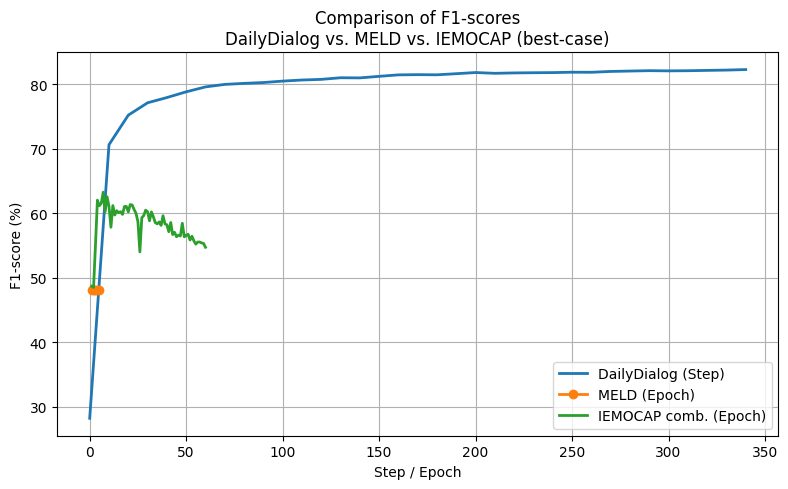
\includegraphics[width=\linewidth]{images/comparaison_en.png}
        \caption{Cross-dataset comparison}
        \label{fig:comparaison_en}
      \end{minipage}\hfill
      \begin{minipage}[t]{0.48\columnwidth}
        \centering
        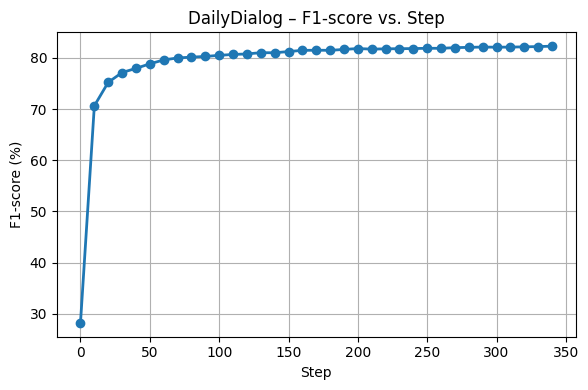
\includegraphics[width=\linewidth]{images/daily_dailog_en.png}
        \caption{F$_1$ vs.\ training step on DailyDialog}
        \label{fig:daily_en}
      \end{minipage}
  
      \vspace{0.5em}
  
      % deuxième ligne
      \begin{minipage}[t]{0.48\columnwidth}
        \centering
        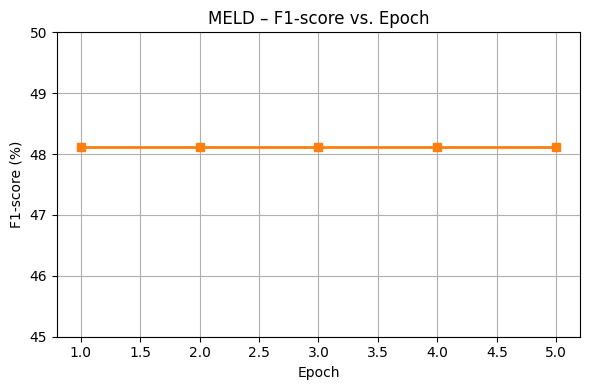
\includegraphics[width=\linewidth]{images/meld_en.png}
        \caption{Performance on MELD}
        \label{fig:meld_en}
      \end{minipage}\hfill
      \begin{minipage}[t]{0.48\columnwidth}
        \centering
        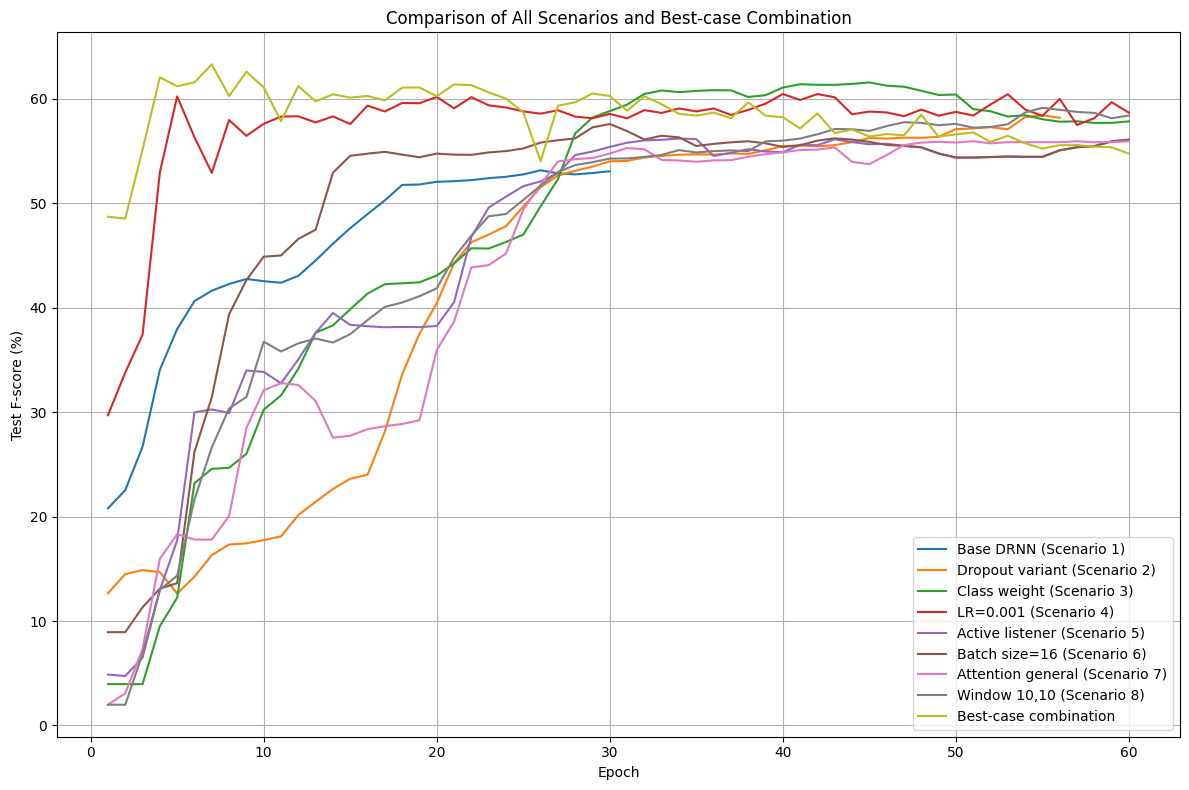
\includegraphics[width=\linewidth]{images/scenario_en.png}
        \caption{IEMOCAP – scenario comparison}
        \label{fig:scenario_en}
      \end{minipage}
  
      \caption{Summary of all experimental results}
      \label{fig:all_results_en}
    \end{figure}
  

  \end{column}

  % Third column
\begin{column}{0.36\textwidth}

    \begin{block}{Conclusion}
      \textbf{Summary}:
      \begin{itemize}
          \item Reproduction validated: <1\% gap on IEMOCAP.
          \item Strong sensitivity to hyperparameters (dropout, context window).
          \item CPU limits: memory overload on EmoryNLP and MELD.
      \end{itemize}
      
      \vspace{0.5em}
      \textbf{Perspectives}:
      \begin{itemize}
          \item Memory optimization: graph filtering, dynamic GCNs.
          \item Multimodal fusion: adding audio and visual streams.
          \item Interpretability: use of GNNExplainer.
      \end{itemize}
    \end{block}

    \begin{block}{References}
      \footnotesize
      \begin{itemize}
        \item Ghosal et al. (2019), \textit{DialogueGCN}, EMNLP-IJCNLP.
        \item Majumder et al. (2019), \textit{DialogueRNN}, ACL.
        \item Busso et al. (2008), \textit{IEMOCAP corpus}.
        \item Poria et al. (2019), \textit{MELD dataset}.
        \item Li et al. (2017), \textit{DailyDialog dataset}.
      \end{itemize}
    \end{block}
  \end{column}

\end{columns}
\end{frame}
\end{document}
